\documentclass[12pt, letterpaper]{article}
\usepackage{amsmath}
\usepackage{graphicx}

\title{The Monin-Obukhov Module for FMS}
\date{}
\author{}

\begin{document}
\maketitle

\section{The Similarity Theory}

Monin-Obukhov similarity (MOS) theory is the standard method for
computing surface fluxes from the lowest level winds, temperatures and
tracer mixing ratios in GCMs.  The lowest level is assumed to lie
within the ``surface layer'' in which turbulent fluxes have negligible
vertical variation, and in which MOS assumes that the wind and
buoyancy profile are a function only of the surface stress, the
surface buoyancy flux, and the height z.  A good reference is
\begin{quote}
Garratt, J. R. ``The Atmospheric Boundary Layer'', Cambridge University Press, 1992
\end{quote}

\subsection{Scales}

The surface stress provides a velocity scale, $u_*$, defined so that
the magnitude of the surface stress $\tau$ is given by
\begin{equation}
  \tau = \rho_s u_*^2
\end{equation}
where $\rho_s$ is the surface air density.  The upward surface
buoyancy flux $B$ can then be used to define a buoyancy scale, $b_*$,
\begin{equation}
  B = \rho_s u_* b_*
\end{equation}

In the atmosphere, if one ignores the virtual temperature effect, the
buoyancy can be taken to be
\begin{equation}
  b = g \frac{(\Theta - \Theta_0)}{\Theta_0}
\end{equation}
where $\Theta$ is the potential temperature and $\Theta_0$ is a
constant reference value, which can be chosen equal to the surface
value.  For a hydrostatic atmosphere,
\begin{equation}
  \frac{1}{\Theta} \frac{\partial \Theta}{\partial z} = \frac{1}{T} \frac{\partial T}{\partial z} + \frac{g}{c_p}
\end{equation}
so, instead of potential temperature, one can equally well use the dry
static energy divided by $c_p: T + g z/c_p$.  To include virtual
temperature effects, one replaces $T$ or $\Theta$ by the virtual
temperature or virtual potential temperature.  The effects of the
humidity difference between the surface and the lowest model level can
be as large as the temperature difference over the tropical oceans,
when computing buoyancy gradients.

This scaling for the buoyancy is inappropriate in the
``free-convective limit'' in which stress, or $u_*$, vanishes but
there is still a non-zero buoyancy flux.  We return to the question of
the free-convective limit of MOS theory below.

The units of buoyance are $[meters]/[sec]^2$, so one can create a
length scale from $u_*$ and $b_*$,

\begin{equation}
  L = -u_*^2/(\kappa b_*)
\end{equation}

The inclusion of $\kappa =$ von Karmans' constant is conventional.  $L$ is
referred to as the Monin-Obukhov length.  With this sign conventions,
$L$ is positive under stable conditions, in which $B < 0$ (heat flux into
the surface).  Roughly speaking, for $Z < |L|$ the turbulence is
primarily driven mechanically and for $Z > |L|$ it is primarily driven
by buoyancy.  Mechanically driven turbulence always wins out close
enough to the surface, as long as the stress is non-zero.

\subsection{The neutral case}

In the neutral case, $b_* = 0$, and the wind shear is assumed be a
function only of the stress, $u_*$ and the height above the surface
$z$.
\begin{equation}
  \frac{\partial u}{\partial z} = \frac{u_*}{\kappa z}
\end{equation}
This equation can be thought of as defining $\kappa$, which is assumed
to be a universal constant.  From laboratory experiments and
atmospheric observations, the value of $\kappa$ is about 0.4.
Integrating, we obtain the famous logarithmic ``law of the wall'':
\begin{equation}
  u(z) = \frac{u_*}{\kappa} \ln \left( \frac{z}{z_0} \right)
\end{equation}
where $u$ is the wind component if the direction of the surface
stress, and $z_0$ is the ``roughness height'', defined as the height
at which the logarithmic profile would yield zero wind.  (The turning
of the wind is assumed to be negligible within this surface layer.)
The roughness height is the key parameter describing the macroscopic
effects of the surface type on the stress.

The ``neutral drag coefficient'', given the flow at height $z_n$,
$C_n(z)$, is defined so that, in the neutral case, the surface stress
vector is given by
\begin{gather}
  \tau = \rho_s C_n |\mathbf{v}| \mathbf{v} \\
  \frac{|\tau|}{\rho_s} = u_*^2 = C_n(z) |\mathbf{v}(z)|^2
\end{gather}
so that
\begin{equation}
  C_n(z) = \left[\frac{\kappa}{\ln\left(z/z_0\right)}\right]^2
\end{equation}
The neutral drag coefficient is a function of the height at which the
winds are supplied.  Given the roughness height and the height $z$ of
the specified wind, we have simple expressions for the drag
coefficient and surface stress.  (Quite often in meteorology, the term
``surface winds'' refers to the winds at a height of 10m, and drag
coefficients are quoted with the assumption that they refer to winds
at this height.)

\subsection{Stratification}

In the stratified case, the key assumption in MOS is that the profile
can also depend on $\zeta \equiv z/L$.  It is conventional to write
\begin{equation}
  \frac{\kappa z}{u_*}\frac{\partial u}{\partial z} = \Phi_m(\zeta)
\end{equation}
where $\Phi_m$ is presumed to be a universal function of $\zeta$.
$\Phi_m \rightarrow 1$ as $\zeta \rightarrow 0$, so that the
logarithmic profile is achieved as the surface is approached.
Integrating from $z_0$ to $z$, we find
\begin{equation}
  u(z) = \frac{u_*}{\kappa}\big(\left(F_m(z/L\right)-F_m\left(z_o/L\right)\big)
\end{equation}
where
\begin{equation}
  F_m(\zeta) \equiv \int \zeta^{-1}\Phi_m d\zeta
\end{equation}
The assumption is that $z_0$ is not a function of stability, which is
plausible as long as $z_0 \ll |L|$.

The problem now becomes that of generating the simultaneous surface
fluxes of buoyancy and momentum from the values of $u$ and $b$ at some
height $z$; the determination of the wind profile is coupled to that of
determining the buoyancy profile.

Therefore, by the same scaling argument, one writes the buoyancy profile as,
\begin{equation}
  \frac{\kappa z}{b_*} \frac{\partial b}{\partial z} = \Phi_b(\zeta) \label{eq:bprofile}
\end{equation}
Integrating as before,
\begin{equation}
  b(z) - b(0) = \frac{b_*}{\kappa}\big(F_b\left(z/L\right) - F_b\left(z_b/L\right)\big)
\end{equation}
where $z_b$ is the roughness length for buoyancy, defined so that $b$
would take on its surface value at $z_b$.  In the neutral limit, both
$F_m$ and $F_b$ should equal $\ln\left(\zeta\right)$.

In general, there is no reason to expect $z_0$ and $z_b$ to be the
same.  Typically $z_0 > z_b$ because momentum can be transferred to
the surface through pressure forces as well as molecular viscosity,
whereas temperature and humidity must be transferred by molecular
diffusion at the surface (except when there is sea spray etc.).  One
sometimes uses the notation
\begin{equation}
  n \equiv \ln\left(z_0/z_b\right)
\end{equation}
For example, Garratt suggests that $n \approx 2$ over typical land
surfaces.

\section{Solving For Surface Fluxes}

Given the form of the stability functions $F_m$ and $F_b$, one can
obtain a consistency condition by computing $L$
\begin{equation}
  L = -u_*^2/(\kappa b_*) = \frac{u(z)^2\big(F_b\left(\zeta\right) - F_b\left(\zeta z_b/z\right)\big)}
    {\big(b(z) - b(0)\big)\big(F_m\left(\zeta\right) - F_m\left(\zeta z_0/z\right)\big)^2}
\end{equation}
of
\begin{equation}
  R_b = \zeta \frac{F_b\left(\zeta\right) - F_b\left(\zeta z_b/z\right)}
    {\big(F_m\left(\zeta\right) - F_m\left(\zeta z_0/z\right)\big)^2} \label{eq:Rb}
\end{equation}
where $R_b$ is the ``Bulk Richardson number'' between the surface and
the height $z$
\begin{equation}
  R_b \equiv \frac{z\big(b(z) - b(0)\big)}{u(z)^2} =
    \frac{g z \big(\Theta_v(z) - \Theta_v(0)\big)}{\Theta_v(0)u(z)^2}
\end{equation}
Eq \eqref{eq:Rb} can then be solved iteratively for $\zeta$, given
$R_b$, $z_0/z$, and $z_b/z$.

Given $\zeta$, one can then compute
\begin{equation}
  u_* = \frac{\kappa |u(z)|}{F_m(\zeta) - F_h(\zeta z_0/z)}
\end{equation}
and
\begin{equation}
  b_* = \frac{\kappa\big(b(z) - b(0)\big)}{F_b(\zeta)-F_h(\zeta z_b/z)}
\end{equation}
These values correspond to the drag coefficients
\begin{equation}
  C_m = \frac{\kappa^2}{\big(F_m(\zeta) - F_m(\zeta z_0/z)\big)^2}
\end{equation}
and
\begin{equation}
  C_b = \frac{\kappa^2}{\big(F_m(\zeta) - F_m(\zeta z_0/z)\big)\big(F_b(\zeta)-F_b(\zeta z_b/z)\big)}
\end{equation}
In implementing this theory, once one has chosen similarity functions,
on has a choice of iterating to a solution whenever it is needed, or
of tabulating the solution for the relevant range of inputs, and,
potentially, fitting the results with easily evaluated functions.
Given that there are three inputs, the typical (but not universal)
choice is to iterate.  If there were only two inputs -- i.e., if one
could assume that the ration of $z_0$ to $z_h$ were fixed, tabulation
and curve fitting would be more straightforward.  In FMS, the solution
is obtained by iteration.

For the purpose of iteration using Netwon-Raphson, we note that the
needed derivative is
\begin{equation}
  \partial R_b/\partial \zeta = R_b\left(\frac{1}{\zeta} + \frac{\Phi_b(\zeta)-\Phi_b(\zeta z_0/z)}{F_b(\zeta)-F_b(\zeta z_b/z)} -
  2\frac{\Phi_m(\zeta)-\Phi_m(\zeta z_0/z)}{F_m(\zeta)-F_m(\zeta z_b/z)}\right)
\end{equation}

\section{The Stability Functions}

Ideally there would be a generally accepted theory for the stability
functions, but no such theory exists, and they are evaluated from
atmospheric field studies.  The forms that receive the most support,
and that are recommended by Garratt, are for the unstable case $\zeta
< 0$,
\begin{gather}
  \Phi_m = (1 - 16\zeta)^{-1/4} \label{eq:stabfuncm} \\
  \Phi_b = (1 - 16\zeta)^{-1/2} \label{eq:stabfuncb}
\end{gather}
and in the stable case $\zeta > 0$,
\begin{equation}
  \Phi_m = \Phi_b = 1+5\zeta \label{eq:stablephi}
\end{equation}
These are considered to have empirical support in the range
$-5<\zeta<1$.

\subsection{The unstable case}

Consider the limit that the mean wind, and therefore, the surface
stress and the friction velocity $u_*$ then to zero.  With the choice
of stability functions presented above, the result will be zero
buoyancy flux as well.  This will be true as long ad $\Phi_b
\rightarrow 0$ more rapidly than $\zeta^{-1/3}$ as $ |\zeta| \rightarrow \infty $.

To see why $\Phi_b \propto |\zeta|^{-1/3}$ is special, look at the
buoyancy profile and ask under what conditions it approaches a
well-defined limit as $u_* \rightarrow 0$.  We can rewrite
\eqref{eq:bprofile} as
\begin{equation}
  \frac{\partial b}{\partial z} = \frac{B}{\kappa u_* z} \Phi_b(\zeta) =
  \frac{B}{\kappa u_* z} \Phi_b \left(\frac{-\kappa z b_*}{u_*^2}\right) =
  \frac{B}{\kappa U_* z} \Phi_b \left(\frac{-\kappa z B}{u_*^3}\right)
\end{equation}
where $B$ is here the buoyancy flux divided by the surface density.
In order for this profile to be well-defined as $u_* \rightarrow 0$
and $\zeta \rightarrow -\infty$, we need $\Phi_b \propto
|\zeta|^{-1/3}$ so that factors of $u_*$ cancel, leading to
\begin{equation}
  \frac{\partial b}{\partial z} \propto \frac{B^{2/3}}{z^{4/3}}
\end{equation}
which is referred to as the free-convection limit.

With the recommended stability function \eqref{eq:stabfuncb} we have
instead $\Phi_b \propto |\zeta|^{-1/2}$ for large $|\zeta|$.  To see that this results in zero buoyancy flux in the free convective limit, we note that in the large $|\zeta|$ limit, we have
\begin{equation}
  B = \frac{\kappa^2 \Delta b|\mathbf{v}|}{F_m(\zeta)F_b(\zeta)}
\end{equation}
where $\Delta b$ is the buoyancy difference between the surface and level $z$ and $\zeta$ is determined by
\begin{equation}
  R_b = \frac{z\Delta b}{|\mathbf{v}|^2} = \frac{\zeta F_b(\zeta)}{F_m(\zeta)^2}
\end{equation}
Eliminating $F_m$ we have
\begin{equation}
  B^2 \propto \frac{z(\Delta b)^3}{\zeta F_b(\zeta)^3}
\end{equation}
If $\Phi_b \propto |\zeta|^{-1/2}$ for large $|\zeta|$, then we also have $F_b \propto |\zeta|^{-1/2}$.  So $B \rightarrow 0$ as $|\zeta| \rightarrow \infty$.

This is unsatisfactory --- either one must use a stability function
that is consistent with the free-convective limit, or one must not
allow the wind speed that is used in the similarity theory to approach
0.  The latter alternative is the choice made in our model and in many
others.  The picture is that in the convective limit, eddies
transporting buoyancy across level $z$ have length scales that scale
not with $z$ but with the depth of the convective layer $h$, which
violates the assumptions of the original similarity theory.  These
eddies produce wind speed perturbations (``gusts'') of magnitude
\begin{equation}
  G = (Bh)^{1/3}
\end{equation}
which is the only velocity scale that one can generate from $B$ and
$h$.  One can now visualize using the similarity theory on smaller
scales than these gusts, implying that the gusts must be included in
the wind speed that is input into MOS.  From the viewpoint of the MOS
module itself, it need not be concerned with the free-convective limit
--- it assumes that the input wind speed will be bounded away from
zero by some theory of ``gustiness''.

The stability functions \eqref{eq:stabfuncm} and \eqref{eq:stabfuncb}
have the property that $\Phi_M^2 = \Phi_h$.  This implies that the
local (as opposed to the bulk) Richardson's number is equal to
$\zeta$, and, in particular, that $Ri$ is a linear function of $z$.
If there were some dynamical argument for this simple structure, it
would help in justifying this choice of stability functions, but we
are not aware of such an argument.

These forms have the convenient property that we can evaluate the
integral stability functions, $F_m$ and $F_b$ analytically.  One
finds, with considerable effort, that (using the notation
$F(\zeta;\zeta_0) = F(\zeta) - F(\zeta_0)$ where $\zeta_0 = z_0/L =
\zeta z_0/z$)
\begin{multline}
  F_m(\zeta;\zeta_0) =
  \ln\left(\frac{z}{z_0}\right) - 2\ln\left(\frac{1+x}{1+x_0}\right) - \ln\left(\frac{1+x^2}{1+x_0^2}\right) + \\
  2\big(\tan^{-1}(x)-\tan^{-1}(x_0)\big)
\end{multline}
where $x \equiv (1-16\zeta)^{1/4}$; while for buoyancy
\begin{equation}
  F_b(\zeta;\zeta_0) = \ln\left(\frac{z}{z_b}\right)-2\ln\left(\frac{1+y}{1+y_b}\right)
\end{equation}
where $y \equiv (1-16\zeta)^{1/2}$.

These expressions are sufficiently costly to compute, especially
$F_m$, that there might be value in using a table look up for them,
even as part of the overall iteration.  At present, they are simply
computed directly from these expressions within FMS.

\subsection{The stable case}

It si not difficult to show that with $\Phi_b \equiv \Phi_m$, and,
therefore, $F_b \equiv F_m$ on the stable side that the drag
coefficients drop to zero close to $Ri_b < 0.2$, given the form
\eqref{eq:stablephi}.  This critical Richardson's number would be
exactly $0.2$ if one set $z_0 = z_h$.  To see this, note that, with
\eqref{eq:stablephi} we have $F_b = F_m = \ln(\zeta) + \beta\zeta$
with $\beta = 5$, so that
\begin{equation}
  R_b = \frac{\zeta}{\ln(z/z_0) + \beta(\zeta-\zeta_0)}
\end{equation}
As $\zeta$ increases, this in bounded above by $R_{crit} =
\beta^{-1}$.  Therefore, as $R_b$ approaches $R_{crit}$, $\zeta
\rightarrow \infty$, and, therefore, $F_m$, $F_t \rightarrow \infty$
as well, implying that the drag coefficients $\rightarrow 0$.

While $0.2$ is close to the $0.25$ stability criterion for linear
Kelvin Helmholtz instability, it is inconsistent with field data to
set the fluxes to zero at this low a bulk Richardson's number.
Intermittent turbulence still exists t higher stability, associated
with breaking gravity waves likely related to inhomogeneities in the
surface whose effects are not representable in terms of a surface
roughness.

Since the value $\beta = 5$ seems to agree with data in the moderately
stable range, one generally modifies $\Phi_b$ and $\Phi_m$ so that
they have this form for small $\zeta$ but allow non-zero fluxes for
larger $Ri_b$.  Different model use various forms for this purpose.
The simplest would seem to be the most desirable.  It is also very
convenient to have a form that allows one to integrate
$\Phi_m(\zeta)/\zeta$ analytically so that one has a relatively simple
expression for $F_m$.  The MOS module has two options:

Version 1 is
\begin{equation}
  \Phi_m = \Phi_b = 1+\zeta\frac{5+\beta\zeta}{1+\zeta} \label{eq:version1}
\end{equation}
This approaches $1+\beta\zeta$ for large $\zeta$ while preserving the
observed small $\zeta$ behavior.  Once can use $\beta$ as a tunable
parameter to modify the poorly understood surface mixing in very
stable conditions.  In the code, the namelist parameter is $rich\_crit
\equiv 1/\beta$.

Version 2, which we now favor, in that it provides additional controls
on the mixing, is piecewise linear
\begin{gather}
  \Phi_m = \Phi_b = 1+5\zeta;\;\; \zeta < \zeta_T \\
  \Phi_m = \Phi_b = 1+(5-\beta)\zeta_c+\beta\zeta;\;\; \zeta >= \zeta_T
\end{gather}
Here $\beta$ controls the critical $Ri$ as before, while $\zeta_T$
controls the point at which a transition is made from the established
stability function for the fully turbulent boundary layer to the
presumably intermittent turbulence at high stability.  With this
version one can generate drag coefficients that are small but non-zero
for a large range of $Ri$ (see the following section).  In the
namelist, $\zeta_T$ is denoted by $zeta\_trans$.

The integrals of $\Phi(\zeta)/\zeta$ can once again be computed
analytically.

\section{Diffusion coefficients}

The profiles of wind and buoyancy obtained in this way can be thought
of as determining diffusivities that would result in these profiles if
vertical diffusion were the only process action -- which the surface
flux similarity theory effectively assumes in any case.  To obtain
this equivalent diffusivity, one can equate the surface flux with the
diffusivity multiplied by the gradient.  In particular, the kinematic
diffusivity for momentum $K_m$ is then
\begin{equation}
  K_m = \frac{u_*^2}{\partial_zu} = \frac{\kappa u_* z}{\Phi_m(z/L)} \label{eq:momentum}
\end{equation}
This diffusivity for buoyancy (i.e. potential temperature or dry
static energy) is
\begin{equation}
  K_b = \frac{u_*b_*}{\partial_z b} = \frac{\kappa u_* z}{\Phi_b(z/L)} \label{eq:buoyancy}
\end{equation}
corresponding to a Prandtl ratio, $Pr \equiv K_m/K_b = \Phi_b/\Phi_m$.

If one's GCM has sufficient vertical resolution to penetrate this
surface layer, and assuming that the GCM is diffusing in the vertical,
then its diffusivity and viscosity should approach these values as the
surface is approached.

In the stable planetary boundary layer above the surface layer, the
diffusivity if GCMs is often modeled as being local in the vertical,
of the form
\begin{equation}
  K = \ell^2\left|\frac{\partial u}{\partial z}\right|
\end{equation}
where $\ell$ is a mixing length.  In the neutral surface layer, we have
\begin{equation}
  K_m = K_b = \frac{u_*^2}{|\partial u/\partial z|} = (\kappa z)^2\left|\frac{\partial u}{\partial z}\right|
\end{equation}
so in this limit, $\ell = \kappa z$.  In the stratified case, we write
\begin{equation}
  \ell = \kappa z f(Ri)^{1/2}
\end{equation}
so that
\begin{equation}
  K = (\kappa z)^2 \left|\frac{\partial u}{\partial z}\right|f(Ri) \label{eq:stratifiedcase}
\end{equation}
In terms of our stability function $\Phi$, assumed to be the same for
momentum and buoyancy, we have for the stratified case
\begin{equation}
  K_m = K_b = \frac{(\kappa z)^2}{\Phi^2}\left|\frac{\partial u}{\partial z}\right|
\end{equation}
Therefore, we can set
\begin{equation}
  f(Ri) = \big(\Phi(\zeta)\big)^{-2} \label{eq:relRiZeta}
\end{equation}
where, we recall, the relationship between $Ri$ and $\zeta$ is
\begin{equation}
  Ri = \zeta\frac{\Phi_b}{\Phi_m^2} = \frac{\zeta}{\Phi}
\end{equation}
given the assumed equality of $\Phi_m$ and $\Phi_b$.  Solving this
last expression for $\zeta$ as a function of $Ri$, one can substitute
into \eqref{eq:relRiZeta} to obtain $f$ as a function of $Ri$.

If one simply used $\Phi = 1 + \beta\zeta$ one would find that
\begin{equation}
  f(Ri) = (1-\beta Ri)^2
\end{equation}
The analogous expression for version 1 involves the positive solution
of the quadratic
\begin{equation}
  (Ri^{-1}-\beta)\zeta+(Ri^{-1}+6)\zeta-1 = 0
\end{equation}
One can then set $K=\Phi^{-2}$, where $\Phi$ is given by
\eqref{eq:version1}.

\begin{figure}[t]
  \centering
  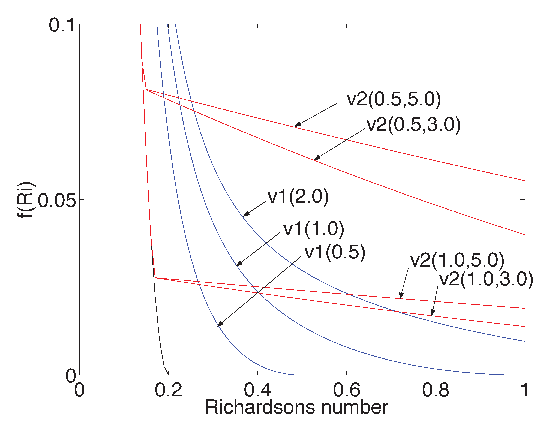
\includegraphics{./monin_obukhov_v1vs2.eps}
  \caption{$f(Ri)$ as a function of $Ri$.  The notation is
    $v1(x)\rightarrow$ version 1 with $x=Ri_{crit}=1/\beta$, $v2(x,y)
    \rightarrow$ version 2 with $x = \zeta_T$ and $y=Ri_{crit}$.}
  \label{fig:f1}
\end{figure}

For version 2 one simply gets
\begin{equation}
  f(Ri) = (1-5Ri)^2;\;\;Ri>Ri_T
\end{equation}
and
\begin{equation}
  f(Ri) = \left(\frac{1-\beta Ri}{1+(5-\beta)\zeta_T}\right)^2;\;\;Ri>Ri_T
\end{equation}
where
\begin{equation}
  Ri_T \equiv \frac{\zeta_T}{1+5\zeta_T}
\end{equation}

One can see from Figure \ref{fig:f1} that version 2 allows one to
match the empirically observed stability function for weakly stable
conditions while still being able to tune the mixing at large
stability, for which there is little empirical guidance and for which
MOS is presumably invalid in any case.  In version 1, if one tries to
increase the mixing at high stabilities one begins to depart
substantially from the empirical relation at weak stability.

In addition to providing a way of matching an interior diffusivity of
form \eqref{eq:stratifiedcase}, these expressions also provide a
useful way of thinking about the strength of the mixing in the surface
layer implied by the similarity profiles.

\section{Implementation Notes}

Four interfaces are provided (see FMS documentation for details)
\begin{itemize}
  \item \textbf{\texttt{mo\_drag}} returns drag coefficients for
    momentum, head, and specific humidity using as input the height
    $z$, the effective wind speed at $z$ (incorporating gustiness),
    and the virtual potential temperature at $z$ and at the surface.
    In addition to the three drag coefficients, output also includes
    $u_*$ and $b_*$
  \item \textbf{\texttt{mo\_profile}} returns the profiles of momentum,
    heat, and specific humidity below height $z$, given the three
    roughness lengths as well as $u_*$, $b_*$, and $q_*$; while $u_*$
    and $b_*$ are available as output from \texttt{mo\_drag}, $q_*$
    must be computed by dividing the evaporation by $u_*$
  \item \textbf{\texttt{mo\_diff}} returns the diffusivities
    consistent with the similarity profiles, as described by
    Eqs. \eqref{eq:momentum} and \eqref{eq:buoyancy}, given $u_*$ and $b_*$
  \item \textbf{\texttt{stable\_mix}} returns the function $f(Ri)$
    described by Eq. \eqref{eq:stratifiedcase}
\end{itemize}

The relevancy of this theory to boundary layer fluxes is typically
limited to $\approx 10\%$ of the planetary boundary layer depth (PBL).
This number seems to arise from the fact that $O(1)$ wind turning and
stress changes occur on the scale of the PBL, so these are likely to
be $O(1/10)$ over the lowest 10 percent of the PBL.)  This provides
strong motivation to place the lowest model level close to the
surface, preferably less than 50 meters.

The assumption is that the differential stability functions for
tracers. such as specific humidity, are the same as those for
buoyancy, or potential temperature.  However, the roughness length for
tracers can be different form that for buoyancy or momentum, so that
the final profiles, and drag coefficients, can be different.  The
monin-obukhov length $L$ and the drag coefficients for momentum and
buoyancy (heat) are functions of the momentum and buoyancy roughness
lengths.  The drag coefficient for tracers is then a function of $L$
and the roughness length for tracer.

The convergence criterion is that the change in $\zeta$ from the
previous iteration $\delta\zeta$, satisfies
$min\big(|\delta\zeta|,|\delta\zeta/\zeta|\big)<1.0\times10^{-04}$.

Convergence of the iteration can be slow when $R_B$ is close to
$R_{crit}$.  To avoid this, $Ri_b$ is arbitrarily set to $Ri_{crit}$
whenever $Ri>0.95R_{crit}$.

The value of von\_Karman's constant is taken from
\texttt{constants\_mod}, as is the value of $g$, required to compute
buoyancy from the potential temperatures input into \texttt{mo\_drag}.

\end{document}
